\documentclass[a4paper]{report}

\usepackage{graphicx}
\usepackage{listings}
% \usepackage{courier} \usepackage{caption}
\usepackage{color}

\lstset{ 
	basicstyle=\normalsize\ttfamily,
    % numbers=left,
    numberstyle=\tiny, 
    numbersep=5pt, 
    tabsize=2, 
    extendedchars=true,
    breaklines=true, 
    keywordstyle=\color{red},
    % frame=b,
    stringstyle=\color{white}\ttfamily, 
    showspaces=false, 
    showtabs=false,
    xleftmargin=17pt, 
    framexleftmargin=17pt, 
    framexrightmargin=5pt,
    framexbottommargin=4pt,
    % backgroundcolor=\color{grey},
    showstringspaces=false
}

\lstloadlanguages{
         % XML
         Python
 }
 
 
\def\authorname{Joseph Ramsay} 
\def\departmentname{LINZ Data Service}
\def\companyname{Land Information New Zealand}


\title{LDS Replicate - Code Maintenance Notes}

\begin{document}

\maketitle

\section*{Summary} The core of the LDSR script was written to be modular
allowing addition of different OGR formats to be added as needed. This is why we
the majority of functionality for the data processing tasks is undertaken by the
DataStore superclass with format specific exceptions implemented in the
respective driver related subclass.

\subsection*{Structure} The basic class structure of the script was originally
designed around a simple commandline interface. This design was intended to be
perform single layer replications. Later additions have added a GUI and mandated
the addition of a centrally controlled connection pool mechanism,
\lstinline|ConfigConnector.DatasourceRegister|, and threading for progress
tracking. Another addition is an installer and setup wizard.

The Class diagram in Figure~\ref{fig:ClassDiagram} shows the basic structire of
the code. The primary DataStore class performs all feature copying and basic
connection, initialisation and maintenance duties.


\begin{figure}[ht!]
  \centering
  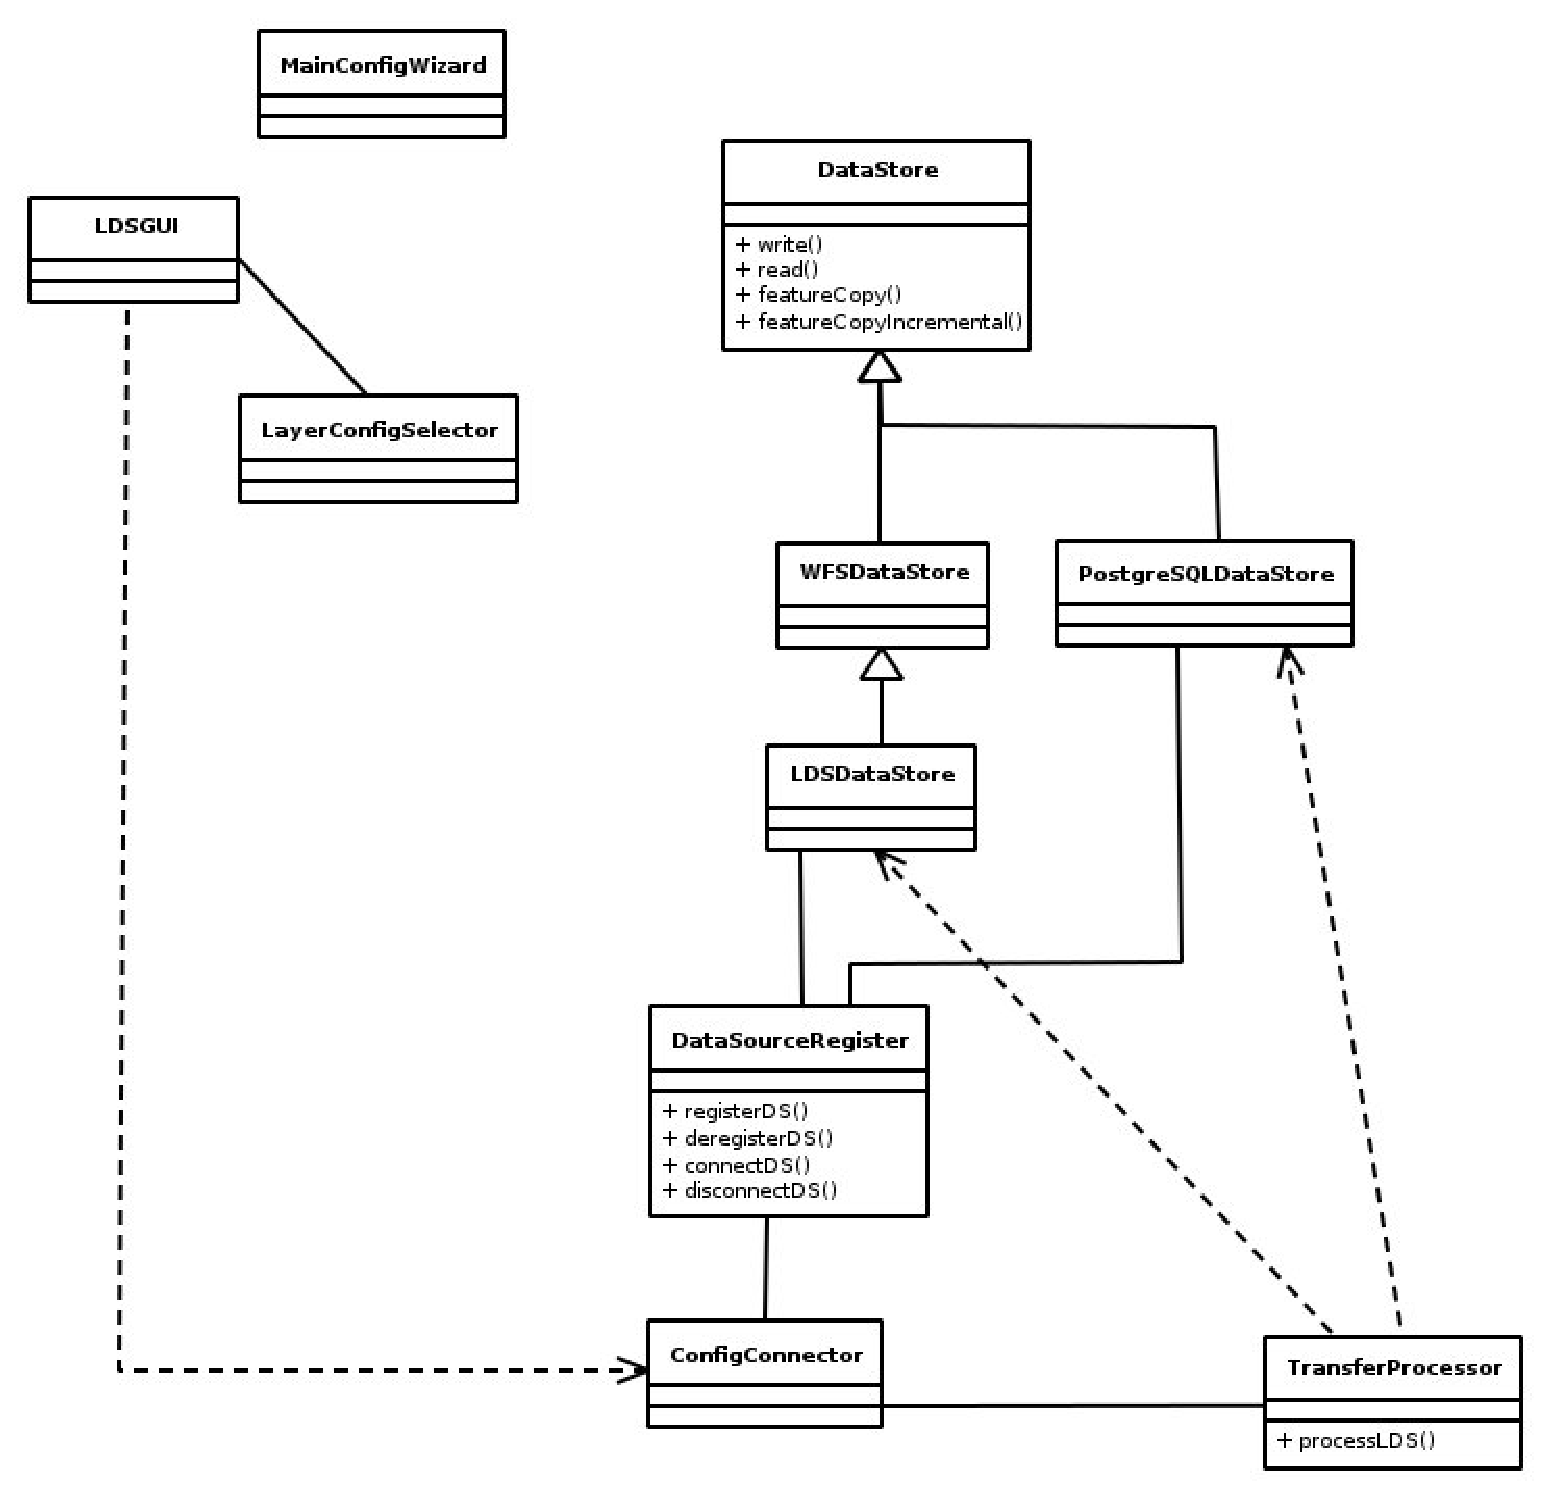
\includegraphics[width=\textwidth]{/home/jramsay/git/LDS/LDSReplicate/doc/LDSR_class.eps}
  \caption{LDSR Class Diagram}
  \label{fig:ClassDiagram}
\end{figure}

Responsibilities that cannot be handled generically are passed off to driver
related subclasses. For example, table index creation is performed directly in
SQL\footnote{GDAL does not provide an API for indexing functions, nor are these
provided in the drivers themselves} and must take into account the different
dialects for their respective databases. the index command in SQL Server is;

\begin{lstlisting}
CREATE SPATIAL INDEX <indexname> ON <tablename> WITH (BOUNDING_BOX=(XMIN=<xmin>,YMIN=<ymin>,XMAX=<xmax>,YMAX=<ymax>))
\end{lstlisting}

In PostgreSQL however that same command takes the form;

 \begin{lstlisting}
CREATE INDEX <indexname> ON <tablename> USING GIST(<spatialcolumnname>)
\end{lstlisting}

Individual DataStore objects are initialised and registered in the
DatasourceRegister ensuring a way to trace connection instances and close
them down if they're not being used. This helps reduce idle connections being
held that prevent connection from external applications.
These connection instances are in turn passed to a \lstinline|TransferProcessor|
(TP) instance to build a replication plan. Depending on provided (stored) dates
the TP checks configuration parameters, layer availability and configures a connection string. It then calls the 
\lstinline|DataStore.write()| method which starts a \lstinline|featureCopy| or 
\lstinline|featureCopyIncremental| operation. Retries and paging are handled at
this stage.
Feature insertion is done by cloning a `partial' feature from the original and
populating it with selected LDS field then using the clone to create a new
feature in the destination.
Incremental requests have the added overhead of having to perform
\emph{update/delete} operations. The additional overhead is created by the need
to match primaty key identifiers between LDS and the destination database.
Because the FID cannot be relied upon to be unique between successive For each
update

\subsection*{Parameter Handling}
Two sets of configurable parameters are maintained. 

\subsubsection*{User Config}
The first of these are
the user configuration settings, including your LDS API key and database
connection strings. These settings are stored in two files, the user editable
\lstinline|user-config-filename.conf| file and the default template file,
\lstinline|template.conf|.\footnote{Either of these files can be written to but
it is good practise to leave the template file with system defaults
and override this in the user config file.} The user configuration file is
created at first run when the Config Wizard is started. It can be added to, or
sections overwritten, by running the Config Wizard again or by editing the file
manually. Parameters are read from these files using
the\lstinline|ReadConfig| module and the  \lstinline|ConfigWrapper| module
handles default substitutions.

\subsubsection*{Layer Config}
The Layer Config file is intended to be mainitained by \lstinline|LDSReplicate|
itself. Its primary function is to store layer processing metadata such as lastmodified
dates, group assignments, output EPSG and CQL specific to a layer.
The Layer Config can be saved as a file on the local machine or in a table in
the destination database. This option is selected at first run by
checking the Internal/(External) option in the first Config Wizard dialog. The
Layer Config file/table is user editable and for more advanced function must be
edited by hand.


\section*{Maintenence Functions}

\subsection*{Destination Module Addition}
In order to build a new DataStore module simply subclass the primary DataStore
class or one of its gerenalised subclasses, \lstinline|WFSDataStore| or
\lstinline|ESRIDataStore|. The functions determining the format of connection
strings, \lstinline|destinationURI()|, \lstinline|sourceURI()| and the function
determining the driver version number \lstinline|versionCheck()| will have to be written. 
Additionally, any functions that make use of raw SQL
to perform an actions will need to be written in their respective driver's
recognised format. \lstinline|buildIndex()| is an example of a function
rewritten sepecifically for differing driver types.
\lstinline|getLayerOptions()| and \lstinline|getConfigOptions()| may also be
added if the driver yoyu are adding has specific config requirements.

Integrating the new module into the existing codebase will require adding extra
members to any driver lists. The primary for driver references can be found in 
\begin{figure}
\begin{lstlisting}
DRIVER_NAMES =
	{'pg':'PostgreSQL',
	'ms':'MSSQLSpatial',
	'sl':'SQLite',
	'fg':'FileGDB'}
\end{lstlisting}
\caption{Supported Drivers}
\label{fig:SupportedDrivers}
\end{figure}

Substituting a new module name (making sure to use the ODR driver name) and
shortcut will take care of many interactions in the code places where this
cannot be factored out include: 
The \lstinline|MainConfigWizard| which will need a new \lstinline|QWizardPage|
where the user can enter new connection details.
The \lstinline|ReadConfig| class will have to have a new function to read these
new configuration parameters.
The \lstinline|ConfigWrapper| class will have to reference the new
\lstinline|ReadConfig| function so that saved user input can be merged
with default values.
To set up those default values a new entry will have to be added to the
template.conf file so that meaningful defaults or user prompts can be returned.


\subsection*{Source (WFS) Module Addition}
Addition of a module doing essentially the same job as the
\lstinline|LDSDataStore| module but pointing at a different address falls
outside the requirements of an LDS replication script but it is likely that extensions to LDS or other providers
using the LDS framework could utilise this script to duplicate data. The obvious
example here is \emph{MfE} who share the LDS platform but identify themselves
through a unique URL. 

Adding a module of this type follows the same principles as adding a
destination module but the immediate superclass of such a module would be
\lstinline|WFSDataStore|. In the case of \emph{MfE}, changes will need to be made to the base URL but modifications may
need to be made in the \lstinline|RequestBuilder| class dpending on the
WFS version being employed and the layer naming scheme.\footnote{While
LDS uses a `v:x\#\#\#' naming scheme a future version (WFS2.0) will employ
`linz-layer:\#\#\#' and \emph{MfE} will be using the prefix `mfe-layer:\#\#\#'}.
Similarly, addition of another departmental client will require changes to the
allowable prefix list.

 \subsection*{Naming Schema Changes}
Without a defined specification some changes have been made in the code
organisation to accomodate future URL format changes, in particular, the layer
naming schema. these changes are realised in the \lstinline|RequestBuilder|
class that attempts to implement format changes as embedded subclasses accessed through
a \lstinline|getInstance()| wrapper.

NB. In the current version, for simplicity and because the naming is unchanged,
\emph{WFS1.0} points to \emph{WFS1.10}


 \subsection*{WFS 2.0}
Anticipating certain changes prompted the creation of the 
\lstinline|RequestBuilder| module but other changes which have not been
explicitly defined will require rewrites. <Ugh! rework>

With \emph{WFS2.0} comes the ability to write requests mixing dependent layers.
For example, although the exact format hasn't been defined, we could request;
\lstinline|cql_filter=layer1 where layer1.geometry intersects layer2.geometry|.
Little needs to be done to support changes to client generated requests but as a
minimum we would have to adjust the \lstinline|LDSUtilities.checkCQL()| constraints or remove this functionality altogether.

\subsection*{Adding User Configuration Parameters}
For user config parameters two sets of configuration parameters are used,
default template parameters and parameters specifically entered by the user. The
\lstinline|ConfigWrapper| class takes care of merging these two values,
overwriting default with user values, when both encountered.
Changing the parameter set requires changes to the
\lstinline|read<Section>Config| method that reads the section being
modified. Data is stored in INI syntax and read using the Python
\lstinline|ConfigParser| module so must be accesed using the provided
\lstinline|get(`section', `option')| method.

\begin{figure}
\begin{lstlisting}
cp = ConfigParser()
cp.read(file_name)
try:
	opt_value = cp.get(`sec_name', `opt_name')
except NoSectionError:
    #No Section Error Message
except NoOptionError:
    #No Option Error Message
return opt_value
\end{lstlisting}
\caption{ConfigParser Get}
\label{fig:ConfigParserGet}
\end{figure}

Parameters additions would require the addition of  a code reading segment along
the lines of the snippet in figure~\ref{fig:ConfigParserGet}. The returned
parameters list would also have to be expanded as would the parameter read
section found in the matching \lstinline|DataStore| initialisation.

\subsection*{Adding Layer Configuration Parameters}
Layer Configuration parameters are accessed in the same way as user
configuration parameters with the added complication that they can also be stored on the
destination database. To read an additional parameter changes need to be made to
the \lstinline|readLayerParameters| method in the
\lstinline|LayerFileReader| class. The companion
\lstinline|LayerDSReader| class that reads from the OGR Feature won't
need an update.
The complication comes when reading from LDS into the Layer Configuration
file/table. The content of this file comes from the WFS GetCapabilities
document which is parsed directly into INI format in the case of local
storage but parsed into an intermediate JSON format for insertion into a
database. The parse here is performed using XSL and is necessarily different for
both the File and Database outputs.

\begin{figure}
\begin{lstlisting}
<xsl:text>"</xsl:text>
<xsl:value-of 
   select="normalize-space(wfs:element-name)"/>
<xsl:text>",</xsl:text>
\end{lstlisting}
\caption{XSL Parser, JSON}
\label{fig:XSLParserJSON}
\end{figure}

In the simplest terms, JSON output relies on array
position and can Figure~\ref{fig:XSLParserJSON}

\begin{figure}
\begin{lstlisting}
<xsl:text>name = </xsl:text>
<xsl:value-of 
   select="normalize-space(wfs:element-name)"/>
<xsl:text>&#xa;</xsl:text>
\end{lstlisting}
\caption{XSL Parser, File}
\label{fig:XSLParserFile}
\end{figure}

 \end{document}